\documentclass[a4paper,11pt,leqno,notitlepage,onecolumn]{article}
%\documentclass[a4paper,11pt,leqno,notitlepage,twocolumn]{article}

\usepackage[latin1]{inputenc}
\usepackage{fontenc}
\usepackage{graphicx}
\usepackage[dvips]{hyperref}
\usepackage{subfigure}
\usepackage{setspace}
%\doublespacing
\usepackage[a4paper]{geometry}
\geometry{top=1in, bottom=1in, left=1in, right=1in}

\begin{document}
\title{PIX: PMaC's Efficient Binary Instrumentor for Linux on x86 Platforms}
\author{Michael Laurenzano, Mustafa M. Tikir, Laura Carrington, Allan Snavely\\
San Diego Supercomputer Center\\
9500 Gilman Drive, La Jolla, CA 92037\\
\it{\{michaell,mtikir,laurac,allans\}@sdsc.edu}}
\date{}
\maketitle

\begin{abstract}
\begin{it}

Binary instrumentation facilitates the insertion of additional code into an
executable in order to observe or modify the behavior of application runs. 
There are two main approaches to binary instrumentation: static and dynamic
binary instrumentation. In this paper we present PMaC's instrumentation toolkit, PIX, 
an efficient static instrumentation toolkit for Linux on x86/x86\_64 platforms. PIX
is similar to  other toolkits in terms of how additional code is inserted. However, it uses function-level
code relocation in order to remedy the difficulty created by the underyling variable-length instruction set. 
Code relocation of this kind allows the reorganization of the application code in such a way that it
can use fast far-reaching constructs to transfer control
from the application to the instrumentation code rather than relying on multiple
jumps or interrupts. Furthermore, the PIX API provides 
tool developers means to insert lightweight hand-coded assembly
rather than relying solely on the insertion of entire instrumentation functions.
Because of these features PIX enables implementation of efficient instrumentation tools. 
The overhead imposed by a simple basic block counting tool created using PIX is an
average of 1.6x less than the overhead imposed by Pin, 4.7x less than the overhead imposed by
DynamoRIO, 7.8x less than the overhead imposed by Valgrind, and 10x less than the overhead imposed by Dyninst.

\end{it}

\end{abstract}

\label{Section:Introduction}
\section{Introduction}
\label{sec:Introduction}

Binary instrumentation toolkits can be used to insert additional code into an
executable in order to observe or modify the behavior of application runs.
Instrumentation toolkits such as Pin\cite{luk2005pin},
Dyninst\cite{buck2000api}, Valgrind\cite{nethercote2007valgrind} and
DynamoRIO\cite{bruening2004efficient} have been widely used to gather
information about application runs. It has been shown that data gathered from
instrumentation tools can be effectively used in guiding hardware and system
design\cite{uhlig1997trace}, program debugging and
correctness\cite{nethercote2007shadow}, program
optimization\cite{romer1997instrumentation}, security
verification\cite{miller-playing}, and performance
modeling/prediction\cite{snavely2001modeling}.

There are two main approaches to binary instrumentation: \textit{static} and
\textit{dynamic} binary instrumentation. Static binary instrumentation inserts
additional information into an executable and generates a persistent modified
executable whereas the dynamic instrumentation inserts additional information
during execution without making any permanent modifications to the executable.
The static instrumentation approach can be advantageous because it usually
results in more efficient executables when compared to the dynamic approach.
This is a result of the fact that static instrumentation introduces only the
instrumentation code itself, which is also included in the text section of the
executable. In dynamic binary instrumentation, additional overhead is introduced
because the instrumentation tool must perform additional tasks such as parsing,
disassembly, code generation, and making other decisions at runtime.

This is simply not an issue with static binary instrumentation tools because all
decisions and actions are taken prior to runtime. The only cost born at runtime
is the direct cost of performing additional instrumentation. Unlike static
instrumentation, dynamic instrumentation uses the program heap for the
instrumentation code and hence, use the data section as text space. However,
static binary instrumentation has disadvantages. It is not possible to
instrument shared libraries unless the shared libraries are instrumented
separately and the executable is modified to use those instrumented libraries.
Static instrumentation also provides less flexibility to tool developers since
any instrumentation code that is inserted persists throughout the application
run while dynamic instrumentation provides the means to delete instrumentation
code when it is not needed \cite{tikir2002efficient}. However, there are cases
where the importance of efficiency is enough to outweigh other shortcomings
\cite{carrington2006performance} so that static binary instrumentation is the
desirable paradigm.   

In this paper we introduce \textbf{P}MaC's \textbf{E}fficient static
\textbf{B}inary \textbf{I}nstrumentation toolkit for \textbf{L}inux on
x86/x86\_64, \textit{PEBIL}. The goal of PEBIL is to provide a toolkit that
enables the construction of instrumentation tools that produce an efficient
instrumented executable. More specifically, PEBIL is designed to generate
efficient instrumented executables for instrumentation tools that require a
large number of instrumentation points because these are the situations where
efficiency is expected to be most impacted. Similar to previous instrumentation
toolkits \cite{buck2000api}, PEBIL instruments the executable by placing a jump
instruction at each instrumentation point in the application which transfers
control to the instrumentation code. This instrumentation code saves program
state, performs tasks requested by the instrumentation tool, restores program
state, and then returns control to the application. A typical binary
instrumentation tool on a platform with fixed-length instructions
\cite{tikir2006pmac} accomplishes initial control transfer by replacing a single
instruction at the instrumentation point with a jump that transfers control to
the instrumentation code. 

When instructions are variable-length, however, this strategy is not always
possible since there may not be enough space to correctly insert such a jump
instruction. To address this, PEBIL relocates and tranforms the code for each
function to ensure that enough space (in the form of \begin{it}nops\end{it}) is
available to hold a full-length branch instruction at each instrumentation
point. This method of function relocation enables transformation of the code so
that it can use longer-range yet efficient jump instructions to transfer control
from the application to the instrumentation code. Similar to Dyninst
\cite{buck2000api}, PEBIL uses the concept of an instrumentation
\textit{snippet}, which is a lightweight hand-written body of assembly code that
can be used to perform instrumentation tasks, rather than relying only on
heavyweight instrumentation functions.

The PEBIL toolkit, along with other accompanying tools and documentation, is
open source and available to the public for download at
\url{http://blind-review-forbids-real-urls.com/}. The distribution includes
several instrumentation tools including a function execution counter, a basic
block execution counter, and a memory address stream collection tool. Each of
these tools is built on top of an API that provides both enough low-level detail
to allow the tool developer to get involved in the details of the
instrumentation and enough high-level capability to allow the tool builder to
ignore these details if he wishes. The three instrumentation tools provided with
the distribution are implemented in less than 600 lines of C++ code. The
remainder of the paper is organized as follows. Section \ref{sec:Overview}
describes the design and implementation of PEBIL. Section \ref{sec:Efficiency}
discusses several aspects of the toolkit that are related to efficiency,
including the function relocation mechanism and the instrumentation snippet.
Section \ref{sec:Results} presents some experiments that expose the performance
penalties imposed by instrumenting applications with PEBIL, as well as a
comparison of PEBIL to other state of the art binary instrumentation toolkits
for x86 including Dyninst, Pin, Valgrind and DynamoRIO. Section \ref{sec:Future}
discusses the future of PEBIL, Section \ref{sec:Related} discusses other popular
instrumentation tools related to PEBIL and Section \ref{sec:Conclusions}
concludes.


\label{Section:Overview}
\section{Design and Implementation}
\label{sec:Overview}

PEBIL is designed to instrument ELF executables that run on the Linux/x86
platform. There are several challenges that must be addressed by any
instrumentation tool in this setting, the largest of which include how to
correctly interpret the information found in the text segment of the application
and how to organize the extra information needed by an instrumentation tool
given the constraints of the binary format and platform.

\subsection{Application Code and Data Discovery}
When compilers explicitly produce a text and data segment for an application,
most default to placing the text segment prior and adjacent to the data segment.
However in any ELF executable, data can also be intertwined with code in the
text segment of the executable for several reasons, including the storage of
branch target locations (e.g. for a jump table that results from a switch
statements) or small data structures that provide convenient and efficient
look-up of data such as identifiers and descriptors. For the sake of correctness
of the executable after instrumentation, it is necessary to identify the parts
of the text section that constitute code and the parts that constitute data.
Mishandling of existing data in the text section as code may result in
instrumented application behavior that differs from the original behavior,
especially if the instrumentation tool modifies or relocates some part of that
data to serve the needs of the instrumentation tool. Such a change in program
behavior may cause outright application failure due to some unintended change in
control flow or some state condition that is checked by the program.
Alternatively, if code is mistakenly treated as data in the text section,
instrumentation might not be inserted or analysis performed that should be
reserved for application data alone.

PEBIL's code discovery algorithm operates on a per-function basis. In order to
determine which parts of the text sections are functions, PEBIL uses the
program's symbol table entries\footnote{The use of the program's symbol table
requires that the program be compiled with debugging information, -g in most
cases} to guide it to each function's entry point. The code discovery algorithm
then consists of two possible phases; control-driven disassembly that is backed
up by linear disassembly. During the control-driven disassembly phase, PEBIL
follows the control flow through a function starting at its entry point. If a
problem is encountered during disassembly such as finding an undefined opcode or
an inconsistent control target, PEBIL assumes that some part of the disassembly
is incorrect and falls back to naive disassembly. During the linear disassembly
phase, each instruction is disassembled in the order it appears in the function
beginning at the function's entry point. If again a problem is found, the
function is tagged as uninstrumentable and the disassembly of the function is
left incomplete and ignored for further instrumentation. This 2-phase
disassembly algorithm correctly disassembled an average of 99.8\% of the basic
blocks for a set of the SPEC CPU2000 Integer benchmarks.

Problems that can be encountered during both phases of code discovery are
situations where an undefined opcode is encountered, where control jumps to the
middle of an instruction PEBIL has already disassembled, or if control leaves
the boundaries of the function via a traditional branch instruction. In most
cases control-driven disassembly is sufficient to disassemble the entire
function, and in most cases this is a straightforward
process because control either falls through to the following instruction or the
location of another possible control target is encoded entirely within the
instruction itself. In more challenging cases an indirect address is used
by a control instruction, where the target resides either at a fixed address
(possibly with some offset), in a register, or at a location given by a
register. The cases where the target computation uses a value from a register 
can be difficult to resolve without runtime
information since the computation of the target address can be arbitrarily
complex and can span function boundaries. Nevertheless, PEBIL performs a
peephole examination of the preceding instructions and can determine the target
address of the branch in most cases.

One of the more common uses of the indirect branch is as part of a jump table.
Fortunately most compilers use relatively simple calculations to determine
targets for jump tables. Often an offset is added to a fixed location to
determine where the data comprising the branch target resides. Therefore, such a
fixed address found in a nearby instruction is treated as the first entry in a
table whose remaining entries are considered to be either addresses or offsets.
PEBIL makes an iterative pass over this table to determine the target address
for each entry in the jump table, stopping when it finds a value in the table
that yields a target address that is outside the function.

\subsection{Instrumentation Code and Data}

Instrumentation generally requires the use of code and data that are not part of
the original executable. In order to insert additional code and data into an
executable, additional space needs to be allocated within the executable in a
way that they will, at load-time, be treated as code and data respectively. Most
compilers produce an ELF executable whose structure is similar to that shown in
Figure \ref{fig:Executable}(a). By convention, most ELF executables use only two
loadable segments and indeed some Linux implementations, such as FreeBSD, allow only
two loadable segments. Thus, it is preferable to incorporate
instrumentation text and data into the existing text and data segments of the
application. 

To accommodate the code and data needed for instrumentation, PEBIL prepends the
instrumentation code to the existing text segment\footnote{The amount of space
allocated prior to the text section is controlled by the linker variable
\_\_executable\_start. There are cases where the system does not provide enough
space prior to the text segment by default, in which case PEBIL comes with a set
of tools that produces a modified linker script on the system that provides up
to 128MB of space.} and appends the instrumentation data to the data segment, as
shown in Figure \ref{fig:Executable}(b). This scheme has the added benefit of
causing no immediate disturbance to the addresses of the original data and most
of the original text of the program.

\begin{figure}[ht]
\centering
\caption{(a) and (b) show that the
text required by an instrumentation tool is prepended to the application text and the data required by an instrumentation
tool is appended to the data application data.}
\label{fig:Executable}
\subfigure[Layout of an unmodified ELF file.]
{
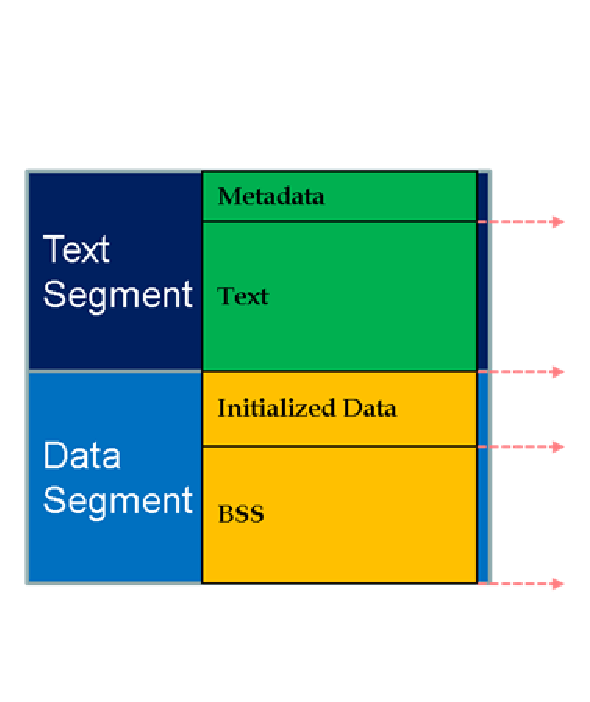
\includegraphics[scale=0.65]{executablep1.eps}
}
\subfigure[Layout of an instrumented ELF file.]
{
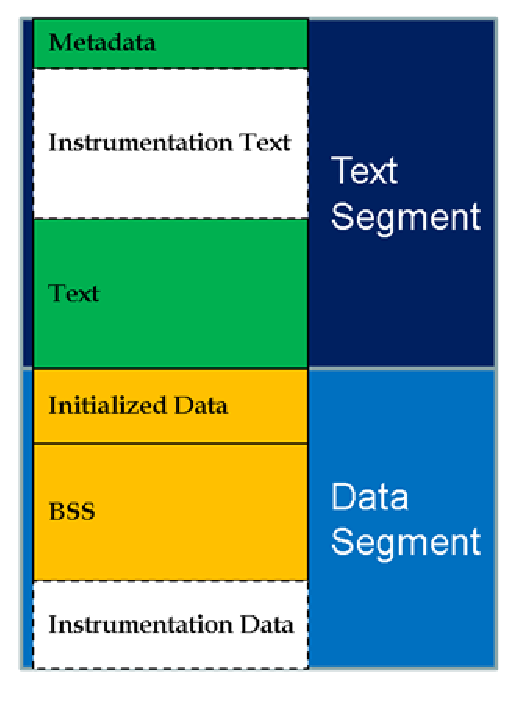
\includegraphics[scale=0.65]{executablep2.eps}
}
\end{figure}

The instrumentation code introduced by PEBIL can be classified by the several
distinct functions it performs. First is code that accomplishes the
instrumentation tasks as well as any bookkeeping code. This code sequence,
called a \textit{trampoline} \cite{buck2000api}, saves any machine state that
will be destroyed, performs the instrumentation task, restores the machine state
after the instrumentation, executes the original instructions that were
displaced by the initial control transfer, and finally restores control to the
original code. When control is transferred from the application to the
instrumentation code, it is necessary to maintain the machine state of the
application to preserve its original behavior. This machine state can contain
anything modified by the instrumentation code, and in practice is usually
limited to a relatively limited set of registers but in some cases includes some
information about the call stack. Since a jump instruction is used at the
instrumentation point, the instrumentation code lacks any information about
where control was transferred from. Hence each instrumentation point uses its
own trampoline so that the location of the instrumentation point can be encoded
into an unconditional branch instruction at the end of the trampoline and
control returns to the application correctly.

Since some instrumentation tools may need additional data to support the
inserted instrumentation code, PEBIL provides mechanisms to insert and
initialize additional data within the executable. The instrumentation text
includes code to initialize this additional data at the beginng of the
application run for use by the instrumentation tool. Recall from Figure
\ref{fig:Executable} that the instrumentation data was appended to the end of
the application's data segment, after the application's uninitialized data
section (BSS section) in order to preserve the application's original addresses.
The initialized data and BSS sections of the data segment are usually
implemented in an ELF executable by declaring the size of the data segment in
the executable to be smaller than the size of the data segment in memory. 

According to the ELF specification \cite{standard1995executable}, the extra part
of any segment whose memory size is greater than its file size should be filled
with zeros by the loader. Hence most programs simply increase the size of the
data segment in memory by the size of the BSS section in order to get an area
that is filled with zeroed, which is reserved for uninitialized data. Since the
area following the BSS section is well-suited for storing additional data for
the instrumentation tool, either the entire data segment's contents, including
the applications BSS section and the instrumentation data, must be included in
the executable file or space can be implicitly reserved and later initialized
using the technique currently employed in most ELF files. Since the BSS section
of an application can be very large and explicit inclusion of its contents into
the executable would bloat the size of the executable file unnecessarily, PEBIL
uses the implicit technique to reserve this section for instrumentation data.
Therefore the instrumentation data is temporarily stored with the
instrumentation text in the executable. This data is then copied to the correct
location in the data segment once execution of the instrumented executable
begins, thus code to accomplish this is included in the instrumentation text as
well.


\label{Section:Efficiency}
\section{Efficiency}

The goal of PIX is to provide a toolkit that enables the construction of
instrumentation tools that produce an efficient instrumented
executable. Specifically PIX is designed to provide efficiency when
the number of instrumentation points is large since cases where the number of
instrumentation points is high are the cases where inefficient instrumentation
has the largest negative impact on application performance. 
In this section we describe some of the important mechanisms used by PIX 
to produce efficient instrumented code.

\label{Subsection:Relocation}
\subsection{Code Relocation}
The use of relocation at the function level in PIX stems from the fact
that instrumentation is being performed statically on a platform that uses a
variable-length instruction set. Because of the variable-length length instructions, it may not always be possible to instrument
an arbitrary point in the executable due to the lack of space for a jump instruction large enough to reach the instrumentation code. 
A typical strategy used by static instrumentation toolkits on platforms with fixed-length instruction sets is to
replace a single instruction at the instrumentation point with a
branch instruction that will transfer control to the instrumentation code. This is fairly straightforward because, by the
definition of a fixed-length instruction set, the instruction being replaced and
the replacing jump instruction have the same length. 
In x86 platforms, a jump instruction that uses a 32-bit offset requires 5 bytes. However, for some
instrumentation points of interest there may not be enough space to hold a 5 byte
jump instruction because the instrumentation point itsself (which might be an instruction or a
basic block) is smaller than 5 bytes. 

Figure \ref{Figure:InstructionSizes} shows a breakdown of the sizes of
instructions for many of the SPEC CPU2000 Integer benchmarks. This figure shows that for these benchmarks,
between 52\% and 74\% of instructions are smaller than 5 bytes. In fact an average of 64\% of instructions
are smaller, which indicates that the the generic technique of replacing 
an instruction with a branch to instrumentation code deserves reexamination because without modification
this technique cannot provide instrumentation to large portions of the application code, which becomes
especially untenable if the instrumentation tool requires many instrumentation points.

\begin{figure}[ht]
\centering
\label{Figure:InstructionSizes}
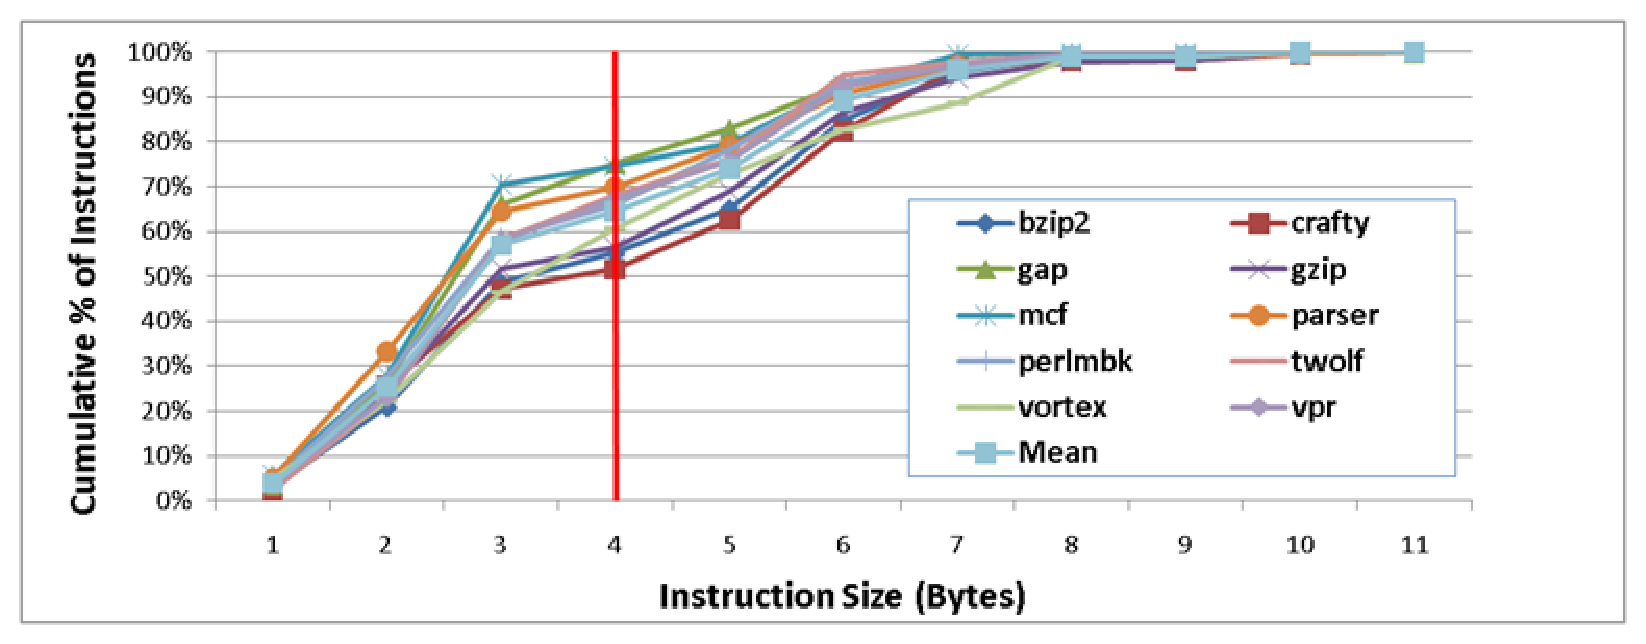
\includegraphics[scale=0.5]{instsize.eps}
\caption{Instruction sizes for several benchmarks presented in a cumulative basis.}
\end{figure}

This leaves two options for transferring control to the instrumentation code.
Either a technique entirely distinct from the idea of using a single
unconditional branch to execute the control transfer must be used or somehow the application code must be altered
in such a way that it can accommodate a single large control instruction that is larger than
the original amount of space available at the instrumentation point. One alternative
technique for transferring control flow to an arbitrary point in the program could be to use a series of branches,
where the instruction at the instrumentation point is a small branch that
transfers control to a larger intermediate branch. This
method is unsatisfactory because the smallest traditional branch instruction available
on the x86 platform is 2 bytes in length, yet there are
instrumentation points with only a single byte available to them. Referring again to figure \ref{Figure:InstructionSizes}, we see
that an average of 4\% of instructions use only a single byte.
Besides, this technique would require additional space to be available in close proximity to the instrumentation points since these
smaller 2-byte branches are also very short reaching. 

%There will also be some overhead associated with setting up a stack frame for the instrumentation function. 
Another option is the method proposed by the BIRD project \cite{nanda2006bird}, which
proposes the use of the single-byte \begin{it}INT3\end{it} instruction when a larger traditional
branch does not fit at the instrumentation point. This instruction is functionally
perfect for static instrumentation because it consumes only a single byte and
allows us to transfer control to an arbitrary location by using the exception handling
facilities provided by the system. We performed a cursory study on this scheme
from an efficiency standpoint to determine whether it was worth further
investigation. On a small benchmark set, our implementation of using
\begin{it}INT3\end{it} only when 5 byte branches do not fit at
the instrumentation point introduces slowdown of at least 100X for
even the simple task of counting the number of executions of each basic block in the code. As one might
expect, this mechanism is unsuitable for efficient instrumentation since the
heavyweight system call conventions are being invoked on a fairly regular basis to
transfer control from the application to the instrumentation code.

In PIX, we use reorganization of the code at the function level so that
there is enough space at every instrumentation point to accommodate a 5 byte
jump. Specifically, the steps used by PIX to relocate the functions and prepare them
for instrumentation are as follows:

\begin{enumerate}
 \item \textit{Function Displacement + Entry Point Linking}
 \item \textit{Branch Conversion}
 \item \textit{Instruction Padding}
 \item \textit{Instrumentation}
\end{enumerate}

Figure \ref{Figure:Relocation} shows an example of this process performed on 
a simple example function in order to prepare the function for instrumentation
that will be inserted at every basic block.

\begin{figure}[ht]
\centering
\caption[Optional caption for list of figures]
{The steps taken in order to prepare a function for instrumentation that will
be inserted at every basic block.}
\subfigure[An unmodified application function.]{
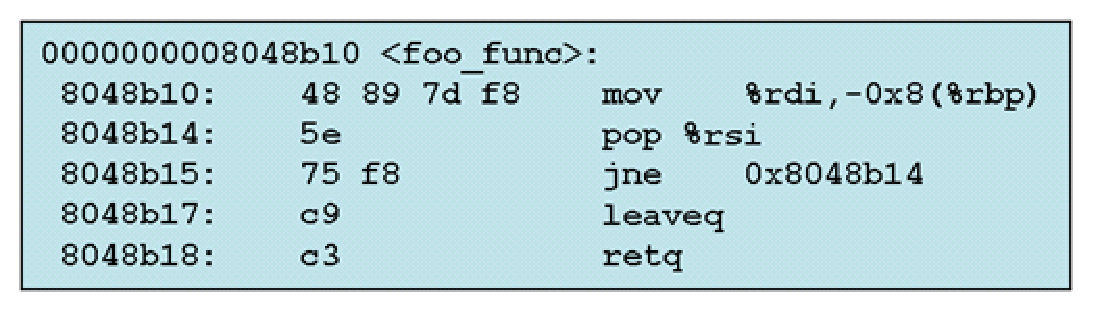
\includegraphics[scale=0.38]{funcp1.eps}
\label{Figure:funcp1}
}
\subfigure[The application function after it has been relocated and the old function entry has been linked to it.]{
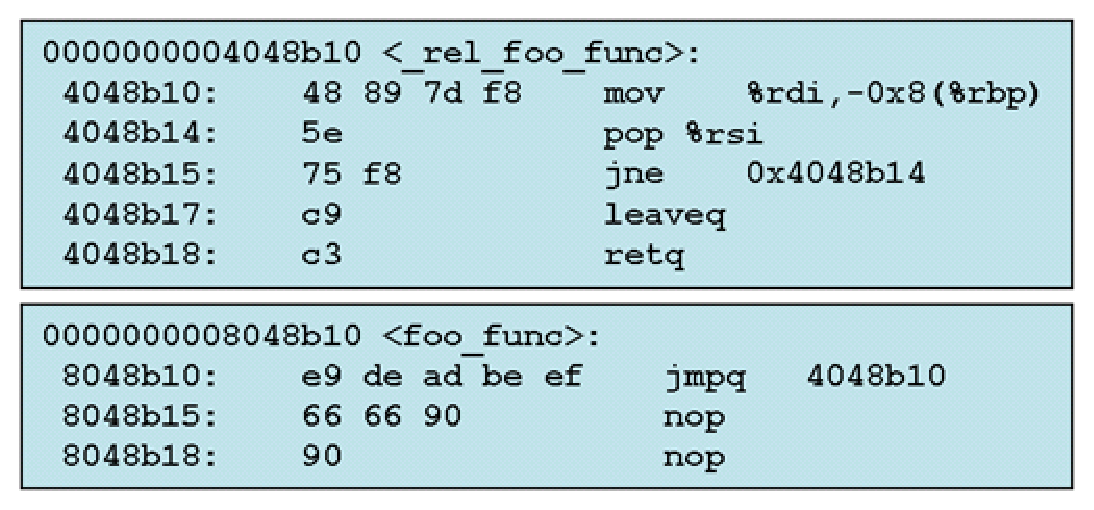
\includegraphics[scale=0.38]{funcp2.eps}
\label{Figure:funcp2}
}
\subfigure[The application function after the branch has been converted to use a 32-bit offset.]{
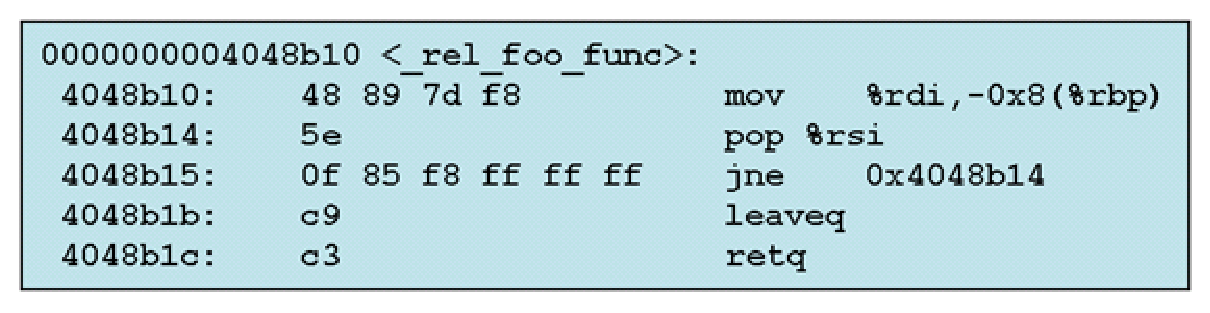
\includegraphics[scale=0.38]{funcp3.eps}
\label{Figure:funcp3}
}
\subfigure[The application function after it has been padded with nop instructions so that each basic block
is large enough to hold a 5 byte jump instruction.]{
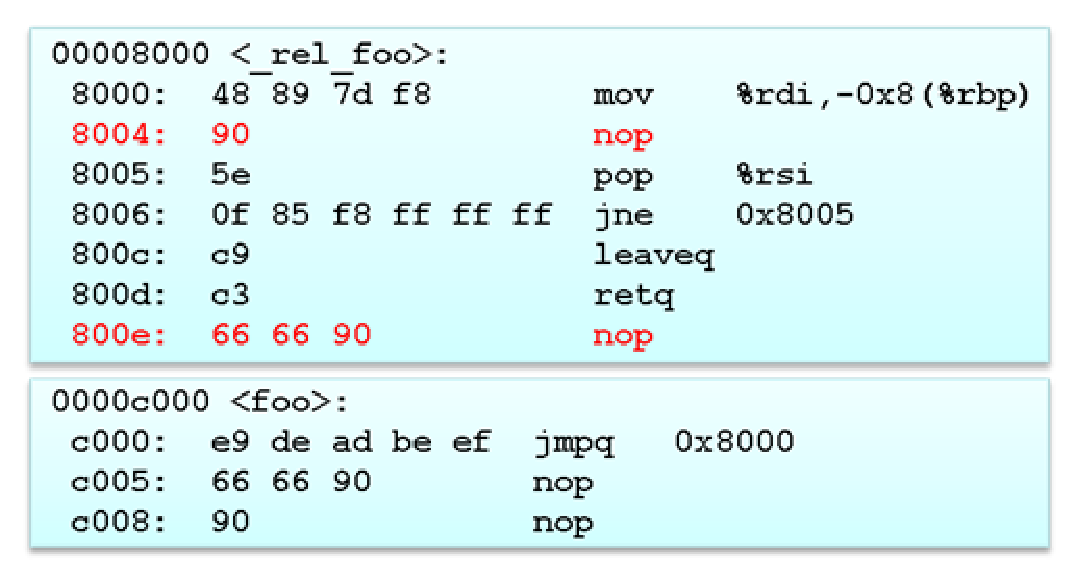
\includegraphics[scale=0.38]{funcp4.eps}
\label{Figure:funcp4}
}
\subfigure[The application function after a single basic block (Basic Block 1) has been instrumented.]{
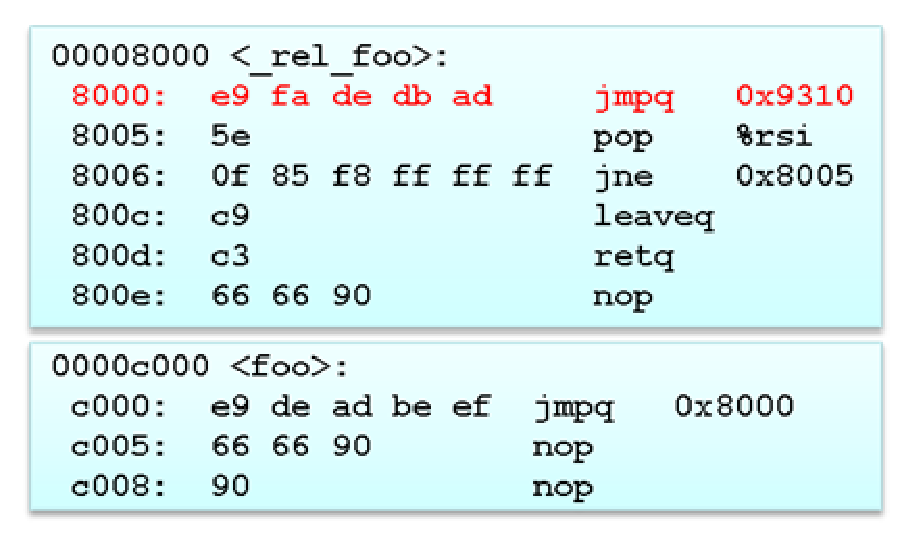
\includegraphics[scale=0.38]{funcp5.eps}
\label{Figure:funcp5}
}
\label{Figure:Relocation}
\end{figure}


Figure \ref{Figure:funcp1} shows a function body prior to any relocation/instrumentation activities.
\textit{Function Displacement + Entry Point Linking} relocates the contents of the entire function to an area of the text section allocated
for the instrumentation. This is done because functions are often packed tightly together. As a result it is generally not possible to keep a function's entry point and
expand its size without disturbing the entry point of another nearby function. The original entry point of the function is then linked to the new location
of the function body by placing an unconditional branch there that transfers control to the new relocated function entry point. 
Linking is done in this fashion because most references to the entry point of a function are in the form of function calls, which
routinely are indirect references (i.e. their value is computed or looked up at runtime) and are difficult to resolve
prior to runtime. See figure \ref{Figure:funcp2}. \textit{Branch Conversion}, shown in figure \ref{Figure:funcp3}, 
converts each short conditional branch in the relocated function to the equivalent
5-byte branch instruction. Since the code is being reorganized in the next step, which may strain the limits of
smaller 8-bit or 16-bit offsets, we convert all branches to use 32-bit offsets so that the targets of each branch
will still be reachable without having the need to make furter changes to the code. Note that there may be some opportunity
here to reduce space by using the smallest branch offset size that accommodates the branch, but currently a single 
unified technique is used in this case to simplify the implementation. Our experiments in Section \ref{Section:Results}, 
however, indicate that the opportunities for improving efficiency for this technique are minimal. \textit{Instruction Padding}, seen
in figure \ref{Figure:funcp4}, pads
each instrumentation point with \begin{it}nop\end{it} instructions so that a 5 byte branch can be accomodated. \textit{Instrumentation} replaces the
some instructions at each instrumentation point with a jump that transfers control to the instrumentation code, which is shown in figure
\ref{Figure:funcp5}.

There are several ways that whole function relocation may adversely affect 
the performance of the instrumented executable independent of the overhead
that will be imposed by the additional instrumentation code. Each function call
now has an extra control interruption associated with it since control must be passed first to the original function entry
point and then to the redirected to the relocated function entry point. In addition it is possible that using 32-bit offsets for every branch rather than
some smaller number of bits has an overhead associated with it. Since the code is being reorganized and expanded, 
we might destroy some positive alignment and size optimizations that the compiler might have made on the instructions in the
function. And finally our technique introduces extra instructions to be executed in the form of nops.

To quantify the impact that function relocation and the other organizational changes have
on the performance of applications, we show the results of experiments
where we generated executables in which functions are relocated, branches are converted to use 32-bit offsets, and 
instruction padding is applied. These experiments show the overhead of the transformations applied to the executable 
in order to prepare it for instrumentation but before any instrumentation code is inserted. The overhead on a set of ten of the 
SPECINT 2000 benchmarks never exceeds 6.5\%, with an average
overhead of just 1.6\%. Thus the basic overhead incurred by the code reorganization in PIX to accomodate all instrumentation points is
well within reason and does not represent a major hurdle for efficiency of the instrumented code.

\subsection{Efficient Instrumentation Snippets}

In most instrumentation tools, the tasks performed by the instrumentation tool are accomplished by allowing the user
to transfer control from instrumentation points in the application to instrumentation functions provided by the user, typically
via a shared library or some object code. Since these instrumentation functions are delivered via a shared library or other
object code, the instrumentation tool developer has the advantage of being able to use a software devlepment toolchain and can
write the code in a language that compiles to the underlying object code. However, such a delivery mechanism is heavyweight due to 
the overhead of a function invocation including saving the complete machine state for all possibles cases in the instrumentation function. In cases where
efficiency is important, it can be more desirable to insert small sequences of assembly code to perform a task and only
save the small subset of machine state that will be affected rather than relying entirely on more heavyweight instrumentation functions and the
more costly state preservation that comes with it.

Some of this state preservation comes in the form of protecting the application call stack from the use of
the call stack by the instrumentation function. The call stack requires protection from the 
instrumentation code during execution because compilers will often optimize a leaf function
by not explicitly creating a stack frame for the local function data to operate in. This optimization is safe for the application because during its
normal execution a leaf function will never call another function and thus its errant stack contents can never be smashed. In the case of an instrumentation
tool that calls an instrumentation function from a leaf, this guarantee no longer holds. Thus, the area above the stack needs to be protected when
an instrumentation function is called from a leaf function. During the disassembly of a function, PIX notes whether it is a leaf function (i.e. whether it contains any call
instructions). Later, during instrumentation, it automatically protects the stack contents for any instrumentation function calls that are made by
incrementing the stack pointer by a fixed safe amount, which has the effect of giving the leaf function a large stack frame while the instrumentation
function's stack frame uses the stack.

Consider the example of an instrumentation point where the desired outcome is to increment a counter that resides in memory. 
In order to accompish this task with an instrumentation snippet, control is transferred to the
instrumentation point's trampoline which will save the platform's flags register, update the counter in memory, restore
the flags register, then transfer control back to the application. Using an instrumentation function, prior to performing
the task the trampoline must save the flags register, any registers used by the function, and
possibly perform some form of stack protection.
It also requires at least 2 more control transfers to enter and exit the instrumentation function. 
Furthermore these control flow transfers generally use the call/return paradigm, which in addition to changing the
application's program counter will also store and retreive information about the function call site onto the stack. 

The use of the instrumentation function is also more likely to pollute the instruction cache more than using a compact
instrumentation snippet. For an instrumentation snippet the application code must contend with the trampoline code
only, whereas using an instrumentation function puts the function code into contention with the other two as well. Hence 
instrumentation functions tend to be more heaviweight than instrumentation snippets. Using snippets rather than functions 
whenever possible allows us to more efficiently gather 
\textit{asynchronous} program information, which intuitively can be thought of as any information that could be dumped to
disk and processed offline. Gao et. al. \cite{gao2005aliter} demostrate that using lightweight instrumentation snippets 
to buffer information which is later processed by more heavyweight instrumentation functions in batches is an efficient
yet entirely lossless way of processing asynchronous program information. The avaialability of instrumentation 
snippets gives tool developers the flexibility to choose either snippets or functions
depending on their performance goals and software engineering needs.


\label{Section:Results}
\section{Results}
\label{sec:Results}

The main design goal of PEBIL is to generate efficient instrumented code. 
To investigate the efficiency of instrumented executables created by PEBIL, we ran several experiments 
on a selection of benchmarks from the the SPEC CPU2000 Integer benchmark suite comprised of
bzip2, crafty, gap, gzip, mcf, parser, perlmbk, twolf, vortex and vpr. All of the experiments are run on a
single core of a quad-core 2.4GHz IA32 Intel Xeon running Red Hat Linux Enterprise 4.1.2 (Linux kernel 2.6.18). 

The first set of experiments quantifies the overhead of the program relocation and 
transformation techniques used by PEBIL and
described in Section \ref{Subsection:Relocation}. 
Recall that this technique adds an additional unconditional
branch execution to each function call in order to relocate the function, extends all of the branches in the code
to use 32-bit offsets, and pads each basic block whose size is fewer than 5 bytes with nops so that a
5 byte jump to the instrumentation code can be inserted. These transformations are performed on our benchmark set 
so that the code is ready for the insertion of instrumentation code but is not actually instrumented. 

Figure \ref{fig:RelocOverhead} presents
the runtime overhead seen in the instrumentation-ready executables as a percentage of the original application runtime.
The figure shows that the maximum overhead due to these modifications is 6.5\%, with an
average overhead of just 1.6\%. Among a set of popular dynamic instrumentation toolkits,
Pin, DynamoRIO and Valgrind, the lowest overhead for running the application within the instrumentation
tool but performing no instrumentation
on the IA32 platform is obtained by using DynamoRIO. DynamoRIO has an average of 38\% overhead and a maximum overhead of 113\% on
our SPEC CPU2000 Integer benchmark set \cite{luk2005pin}. This shows that the 
relocation and transformation method used by PEBIL has a minimal
performance impact on the performance of these benchmarks and thus is a suitable approach as a basis for
producing efficient instrumented code.

\begin{figure}[ht]
\centering
\label{fig:RelocOverhead}
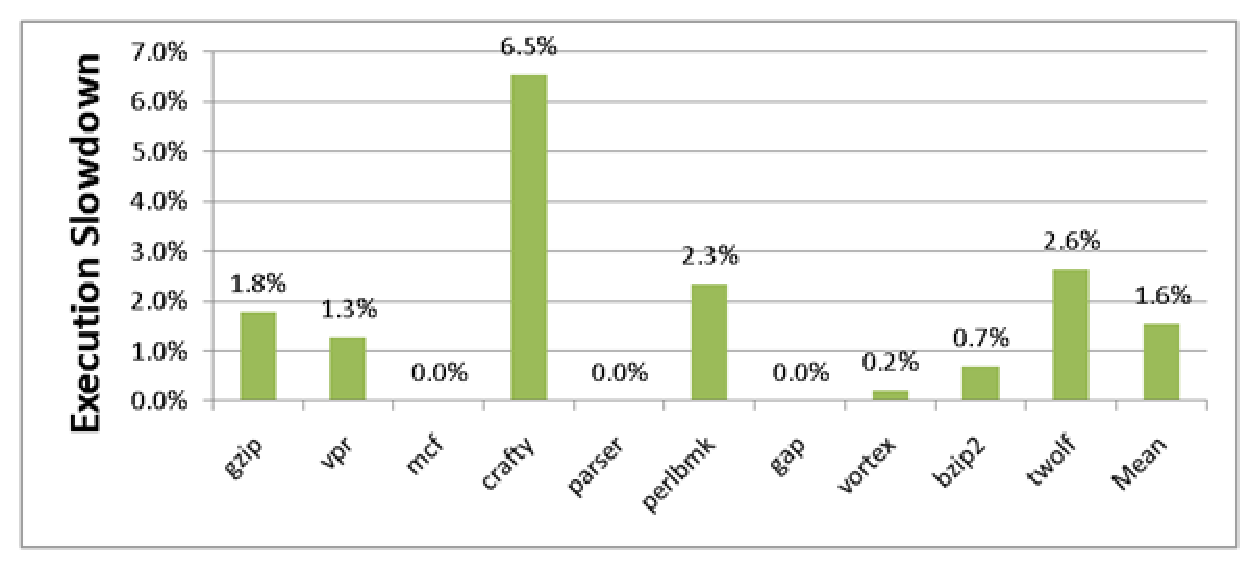
\includegraphics[scale=0.6]{relocperf.eps}
\caption{Application overhead caused by preparing the code for instrumentation but without
any instrumentation inserted.}
\end{figure}

The next set of experiments shows how much overhead is introduced due to counting the
basic block executions in the application. We use this particular instrumentation tool because basic block counting
is an example of an instrumentation tool where we would expect PEBIL to generate efficient instrumented executables
as the number of instrumentation points required is high. Much of the work performed in basic block counting, namely updating a single
counter every time a basic block is encountered, can be done easily using a fast instrumentation snippet rather than
by a full instrumentation function. The counters embodied in the instrumentation snippets must also be
persistent throughout the entire run of the application, which is more suited to a static instrumentation approach
because the static instrumentation does not utilize any resources to determine whether instrumentation can be removed.
The basic block counting instrumentation tool is used to produce an instrumented
executable for each program in our benchmark suite, whose runtime is compared to the runtime of the 
unmodified original executable. The results of these experiments are shown in Figure \ref{fig:ToolOverheads}. 

\begin{figure}[ht]
\centering
\label{fig:ToolOverheads}
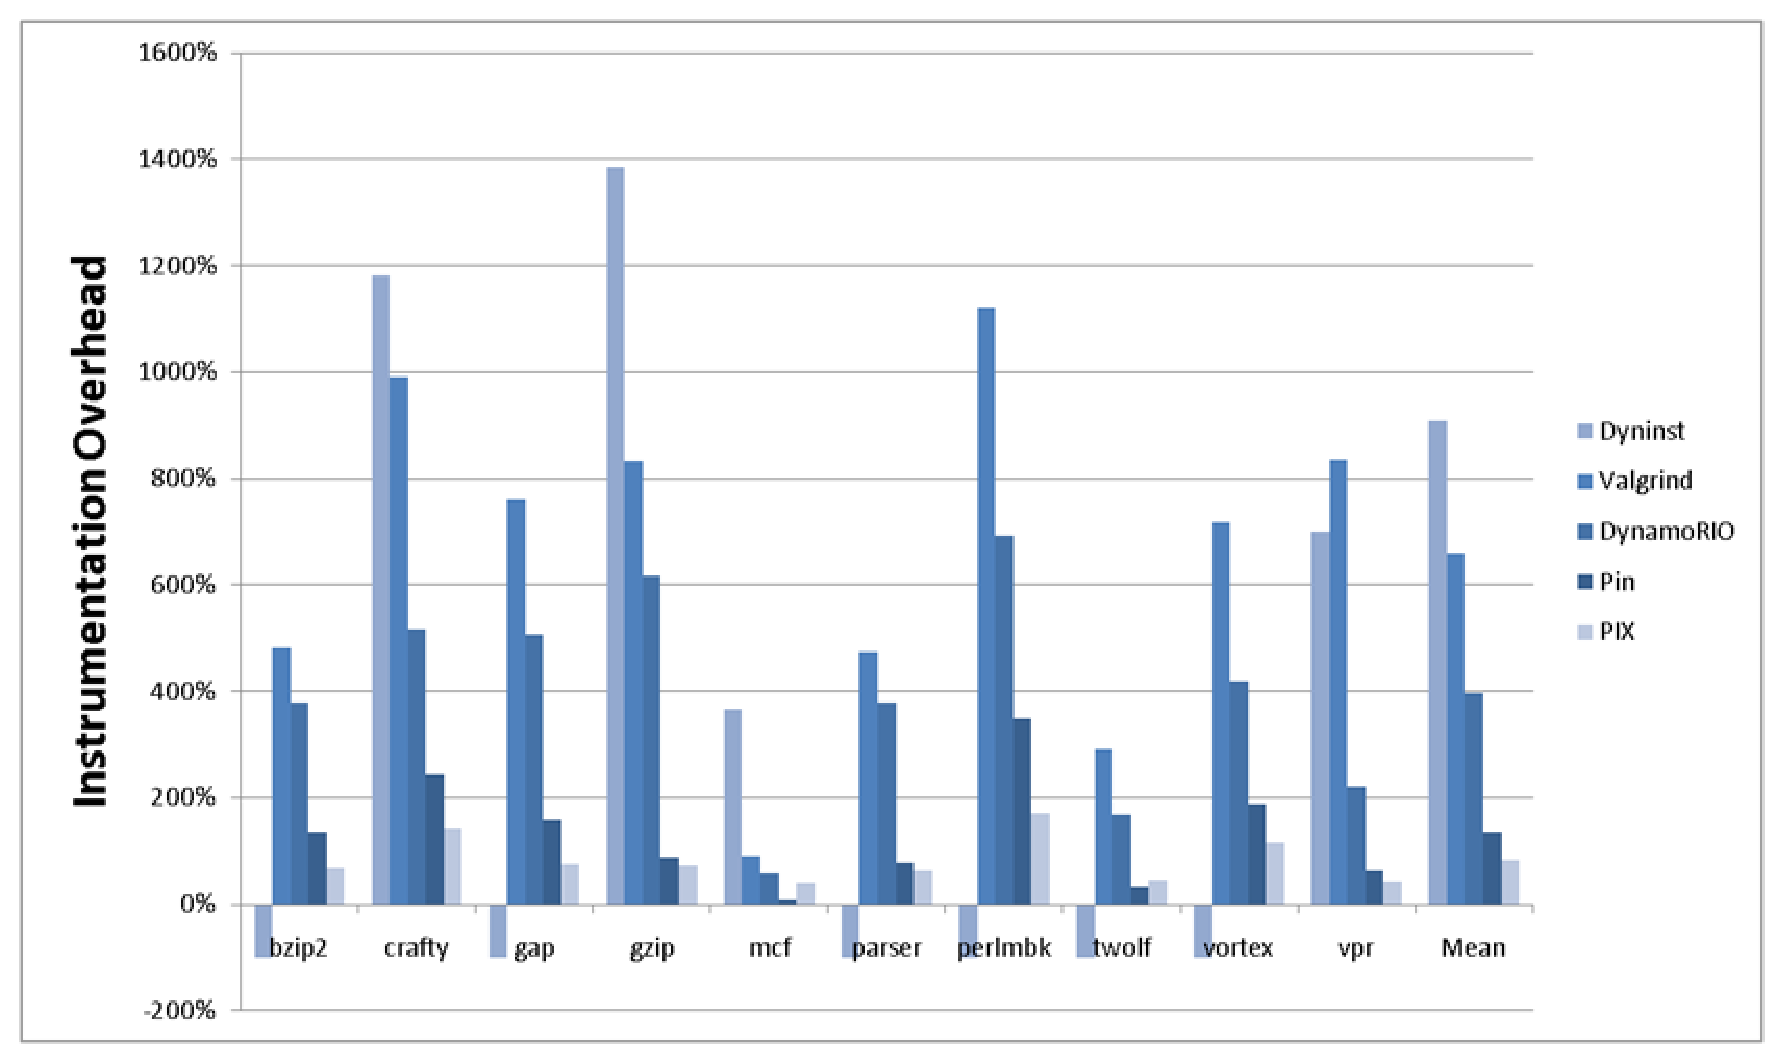
\includegraphics[scale=0.32]{bbcount.eps}
\caption{Performance of several x86 instrumentation tools with basic block counting instrumentation.}
\end{figure}

Figure \ref{fig:ToolOverheads} presents the overhead introduced as a percentage of the original application runtime. The
overhead of PEBIL's basic block counter ranges from 41\%-170\% for the benchmarks tested with an average overhead of 
84\%. More importantly, the figure shows that the overhead introduced by PEBIL instrumentation is significantly 
lower than those introduced by the other instrumentation toolkits available for the x86 platform. 
The average overhead is 135\% for Pin (ranging from 8\%-350\%), 
396\% for DynamoRIO (ranging from 58\%-693\%), 660\% for Valgrind (ranging from 91\%-1120\%), 
and 1936\% for Dyninst (ranging from 367\%-7859\%). Note also that, like PEBIL, the Dyninst
implementation of a basic block counter uses snippet-based instrumentation whenever possible yet
it results in significantly higher overheads than PEBIL.
Our experiments demonstrate that executables instrumented by PEBIL run an average of
51\% faster than the next most efficient instrumentation toolkit for basic block counting, Pin. Furthermore,
Pin uses a variety of optimizations such as tracking eflags bit liveness \cite{luk2005pin} that are currently
unincorporated into PEBIL. We plan to incorporate more optimizations to PEBIL in the future (see Section \ref{sec:Future}) including
several optimizations already in use by Pin, which should further improve the efficiency of the instrumented
executables generated by PEBIL.



\label{Section:Future}
\section{Future Work}
\label{sec:Future}

Despite the success in terms of efficiency, there are several additional techniques
that might make the instrumented code even more efficient in PIX. Because PIX relocates
the text to yeild extra space for the manipulation of the application functions, 
rather than inserting just a branch
that transfers control to the instrumentation code we have the opportunity to inline
the instrumentation code itsself
in order to reduce or eliminate the control interruptions  that otherwise must be taken 
when inserting the instrumentation code.

Currently PIX saves all general purpose registers around each function call and allows the
tool developer to state which registers are saved around instrumentation snippets. For even more efficient instrumentation
snippets, we could automatically detect which registers are killed by the instrumentation code and which are live at the entry point
of the instrumentation code, and automatically save only the ones that are alive. Similarly, we could perform register 
analysis in order to identify the instrumentation points where the machine state doesn't need to be saved around instrumentation functions. 

Finally, similar to Pin, we could perform liveness on the bits of the eflags/rflags register to determine whether the flag registers need to be saved and
restored at each instrumentation point. Optimizations that help PIX avoid saving and restoring state at each instrumentation point 
have the potential to further the overhead associated with instrumentation and we beleive 
that they will further the goal of generating efficient instrumented code with PIX.




\label{Section:Conclusions}
\section{Conclusions}



\bibliography{x86inst}
\bibliographystyle{unsrt}

\end{document}

